
\subsection{Valuation}
\label{meth_val}
The following values were explored for this study: 

\begin{itemize}
	\item the \hyperref[meth_val_aev]{\aev{}}; 
	\item the \hyperref[meth_val_aciv]{\aciv{}}; 
	\item the \hyperref[meth_val_drv]{\drv{} (DRV)};
	\item the \hyperref[meth_val_lsrv]{\lsrv{} (LSRV)}; and 
	\item the \hyperref[meth_val_atdlv]{\atdlv{}}. 
\end{itemize}

\vspace*{10mm}
\begin{centering}
\large\textsc{Need to think about how the methodology and its associated explanation change between utility scale and distributed. Energy may be relatively the same (DAM prices), but would capacity be different? Need to look at capacity credit used for wind turbines in New York \ldots}
\end{centering}
\vspace*{10mm}

An explanation of what these values are intended to represent as well as the methodology used to determine the value follows. The methodology for these values were derived from NYSERDA’s Value Stack Calculator \hl{as were input values}, whenever possible. \cite{nypsc_matter_2019}. % available here: https://www.nyserda.ny.gov/All-Programs/Programs/NY-Sun/Contractors/Value-of-Distributed-Energy-Resources

% ~~~~~~~~~~~~~~~~~~~~~~~~~~~~~~~~~~~~~~~~ /
%  Energy Value
% ~~~~~~~~~~~~~~~~~~~~~~~~~~~~~~~~~~~~~~~~ /


\subsubsection{Avoided Energy Value}
\label{meth_val_aev}
The \aev{} represents the variable costs, such as fuel costs or operating and maintenance costs, avoided by the \hl{distribution utility} when injections of distributed energy offset generation from other units. Whenever a load-serving entity (LSE) seeks to satisfy demand, they typically use generating resources at their disposal in order of their associated variable costs, dispatching least-cost resources first, in order to meet demand as economically as possible. Because resources such as distributed wind and solar PV have no associated fuel costs, they are often the most economic choice for meeting demand when they are generating electricity. Thus exports from DERs will tend to either reduce the need for purchases from electricty markets or will offset generation from more expensive units within the utilitiy's generating fleet. In either case, the net effect of DER exports to the grid is to reduce costs associated with energy procurement for the utility. In the deregulated electricity market of New York, utilities do not own generation and instead purchase the bulk of their energy requirements on the Day Ahead Market (DAM), while using the Real Time Market (RTM) to address imbalances between actual and forecasted demand \textcolor{pink}{textsc{source}}. 

One way to quantify the net \textit{energy} benefits associated DER exports is to measure its ability to reduce the purchases LSEs need to make from the electricity market by meeting demand locally. This is the approach within the Value Stack Calculator, and the \aev{} is calculated as the hourly product of the exports to the grid from the DER and the day ahead market (DAM) price for the NYISO load zone in which the DER exports. For this analysis, the day ahead market prices for the year \hl{2018} were taken from \cite{nyiso_pricing_2020}. Table \ref{table:quantlbmpdam} shows the minimum, $25^{th}$ percentile, median, average, $75^{th}$ percentile, and maximum day ahead market energy prices for the year 2018 across the NYISO load zones considered in the analysis. Figure \ref{fig:boxbmpdam} also graphically shows the distribution of the energy proces. Figure~\ref{fig:expaevplot} shows how the hourly product of the DER exports and the DAM prices are used to yield the \aev{}. 

%In the analysis, the product of the DAM prices and the distributed generation exports are  scaled up by the associated utility transmission and distribution losses to determine the final \aev{}, as generation used to meet demand closer to load experiences fewer losses relative to transmission-sited generation (see \atdlv{}). 

%Equation \eqref{eq:1} mathematically expresses how the \aev{} is determined for a generator \textit{i} located in NYISO load zone \textit{j}. 
%\begin{equation}
%Value_{Energy} (i) = \sum_{\substack{t=0 \\i\;\subseteq\; j}}^{n=8760} \underbrace{Export_{DER} (i,t)}_\text{FOM wind generation} \cdot \underbrace{Energy\;Price_{DAM}(j,t)}_\text{DAM Price} \label{eq:1}
%\end{equation}

\begin{conditionaltable}[!htb]
\centering
    \pgfplotstabletypeset[column type = lccccc, multicolumn names,
      col sep=comma,
	display columns/0/.style={string type, column name=Zone},
	display columns/1/.style={fixed, fixed zerofill, column name=Min},
	display columns/2/.style={fixed, fixed zerofill, column name=$25^{th}$},
	display columns/3/.style={fixed, fixed zerofill, column name=Median},
	display columns/4/.style={fixed, fixed zerofill, column name=Mean},
	display columns/5/.style={fixed, fixed zerofill, column name=$75^{th}$},
	display columns/6/.style={fixed, fixed zerofill, column name=Max},
	every head row/.style={
		before row={\toprule}, 
		after row= & \$/MWh & \$/MWh & \$/MWh & \$/MWh & \$/MWh & \$/MWh \\ 
					\midrule
		},
	every last row/.style={
		after row=\bottomrule
		},
    ]{\quantilelbmpdata}
\caption{Summary Statistics for 2018 NYISO Day Ahead Market Prices by Load Zone. Data Source: \citet{nyiso_pricing_2020}.}
\label{table:quantlbmpdam}
\end{conditionaltable}

\begin{conditionalfigure}[!htb]
  \centering
	  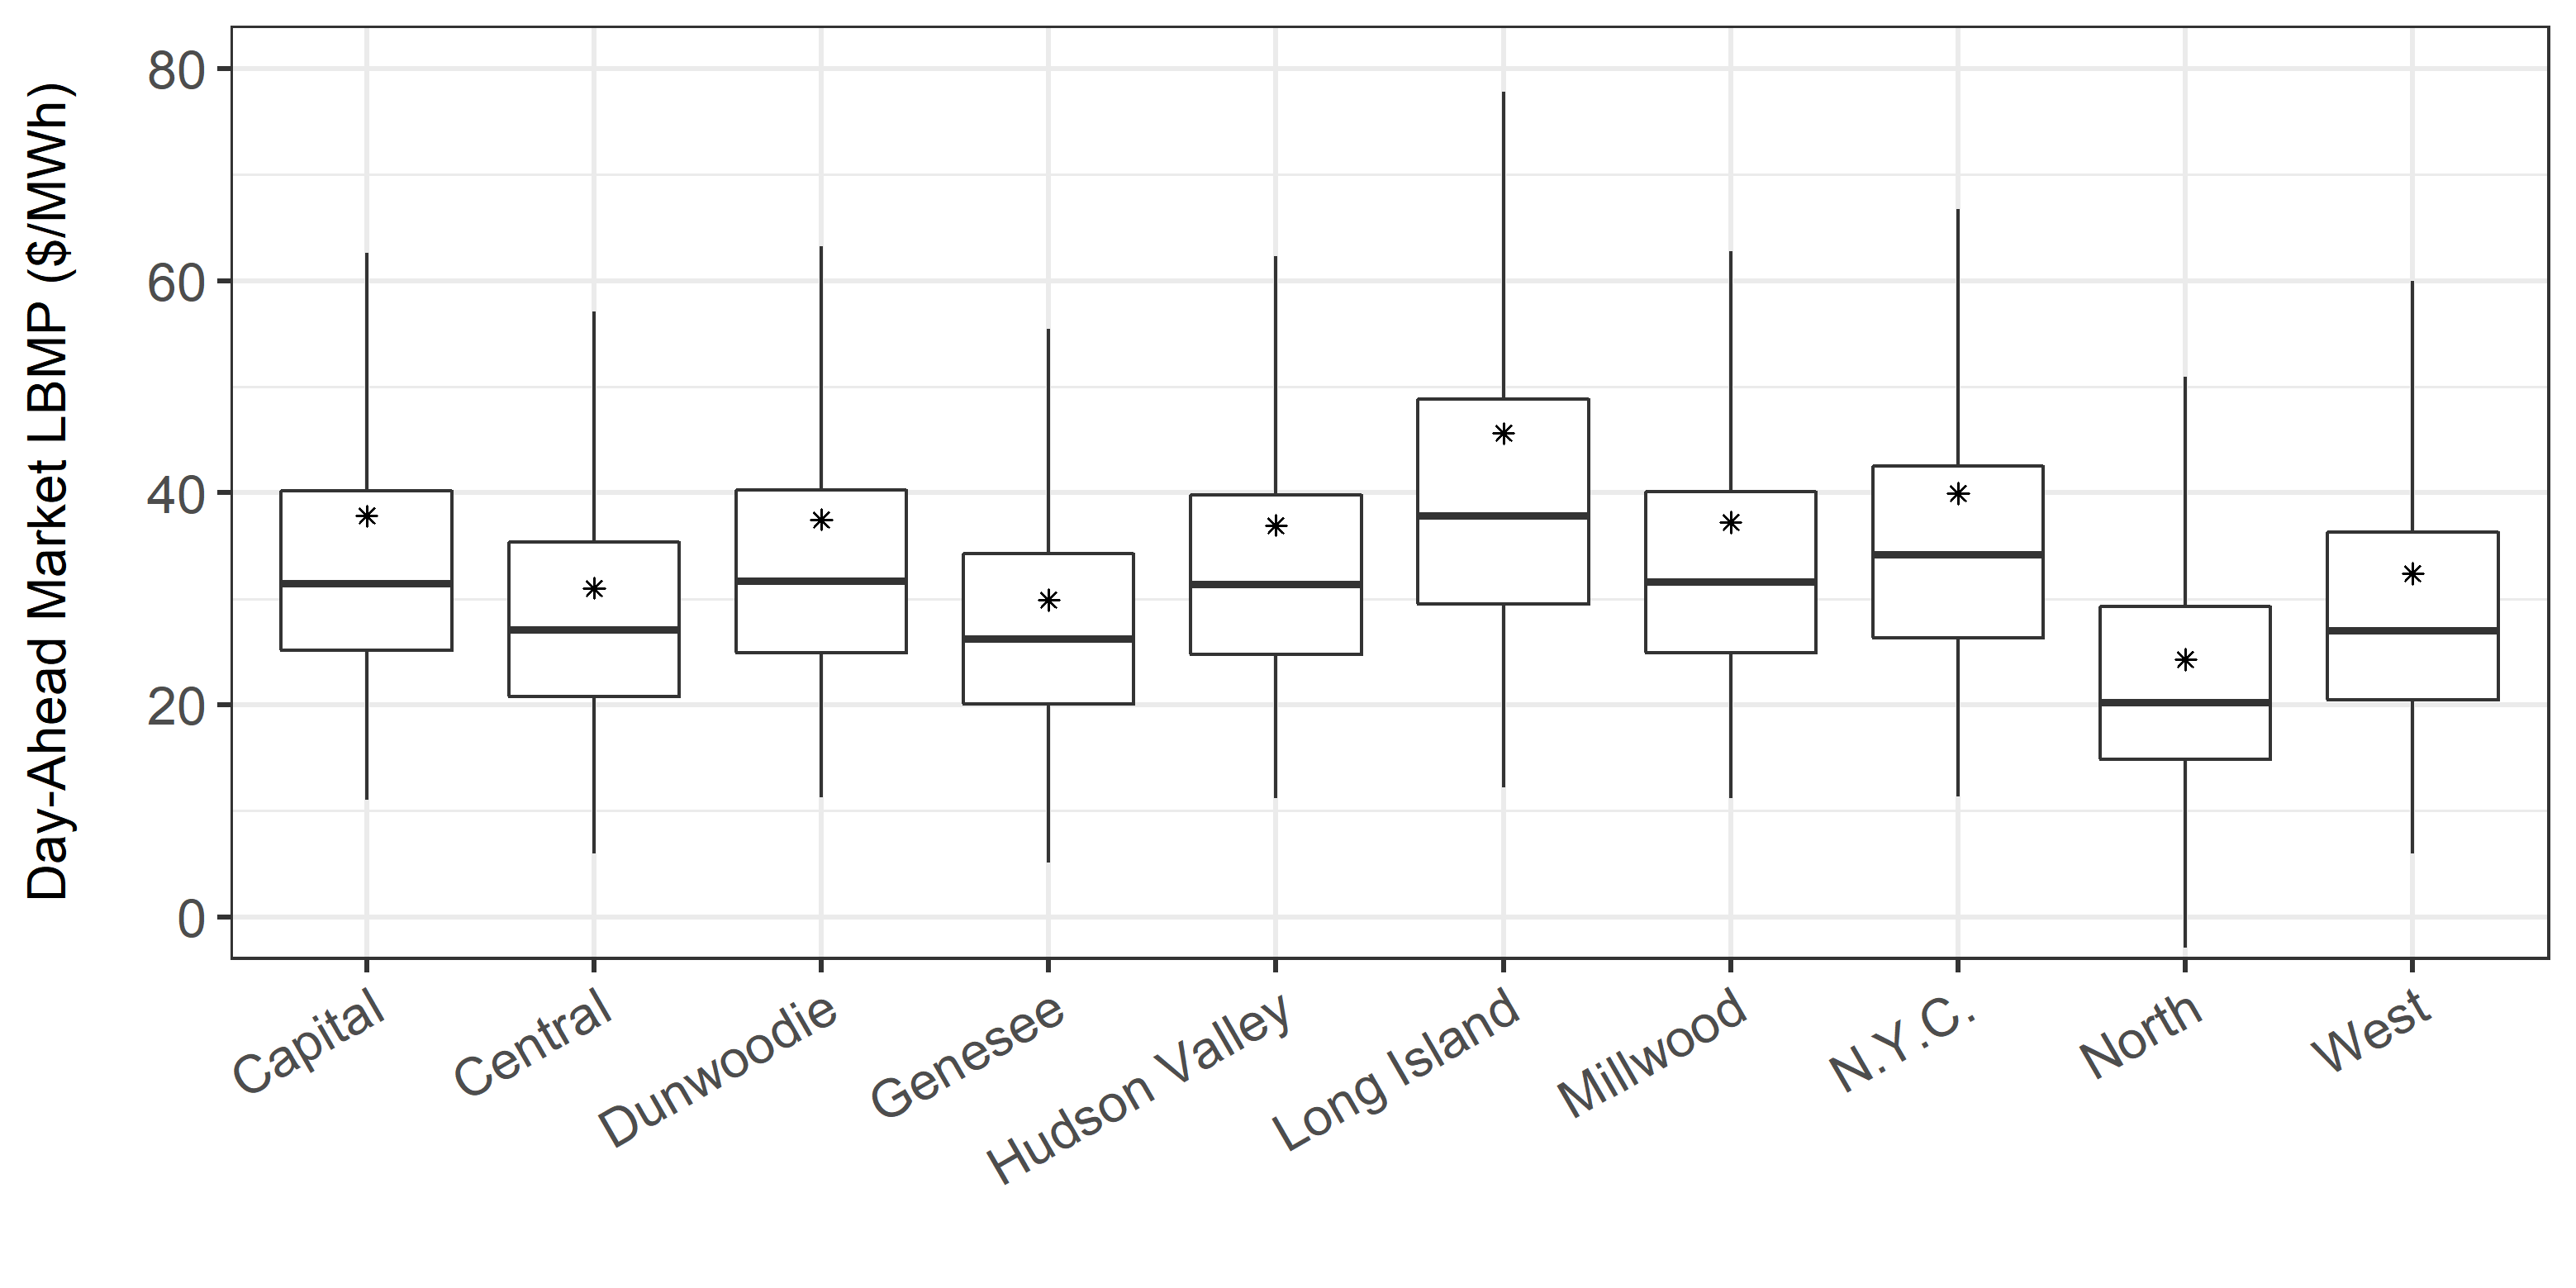
\includegraphics[width=\linewidth]{boxplot_dam_lbmp_prices.png}
	  \caption{Boxplots of LBMP DAM Prices, maximum excluded, mean represented as star. Data Source: \citet{nyiso_pricing_2020}.}
	  \label{fig:boxbmpdam}
\end{conditionalfigure}

\begin{conditionalfigure}[!htb]
  \centering
	  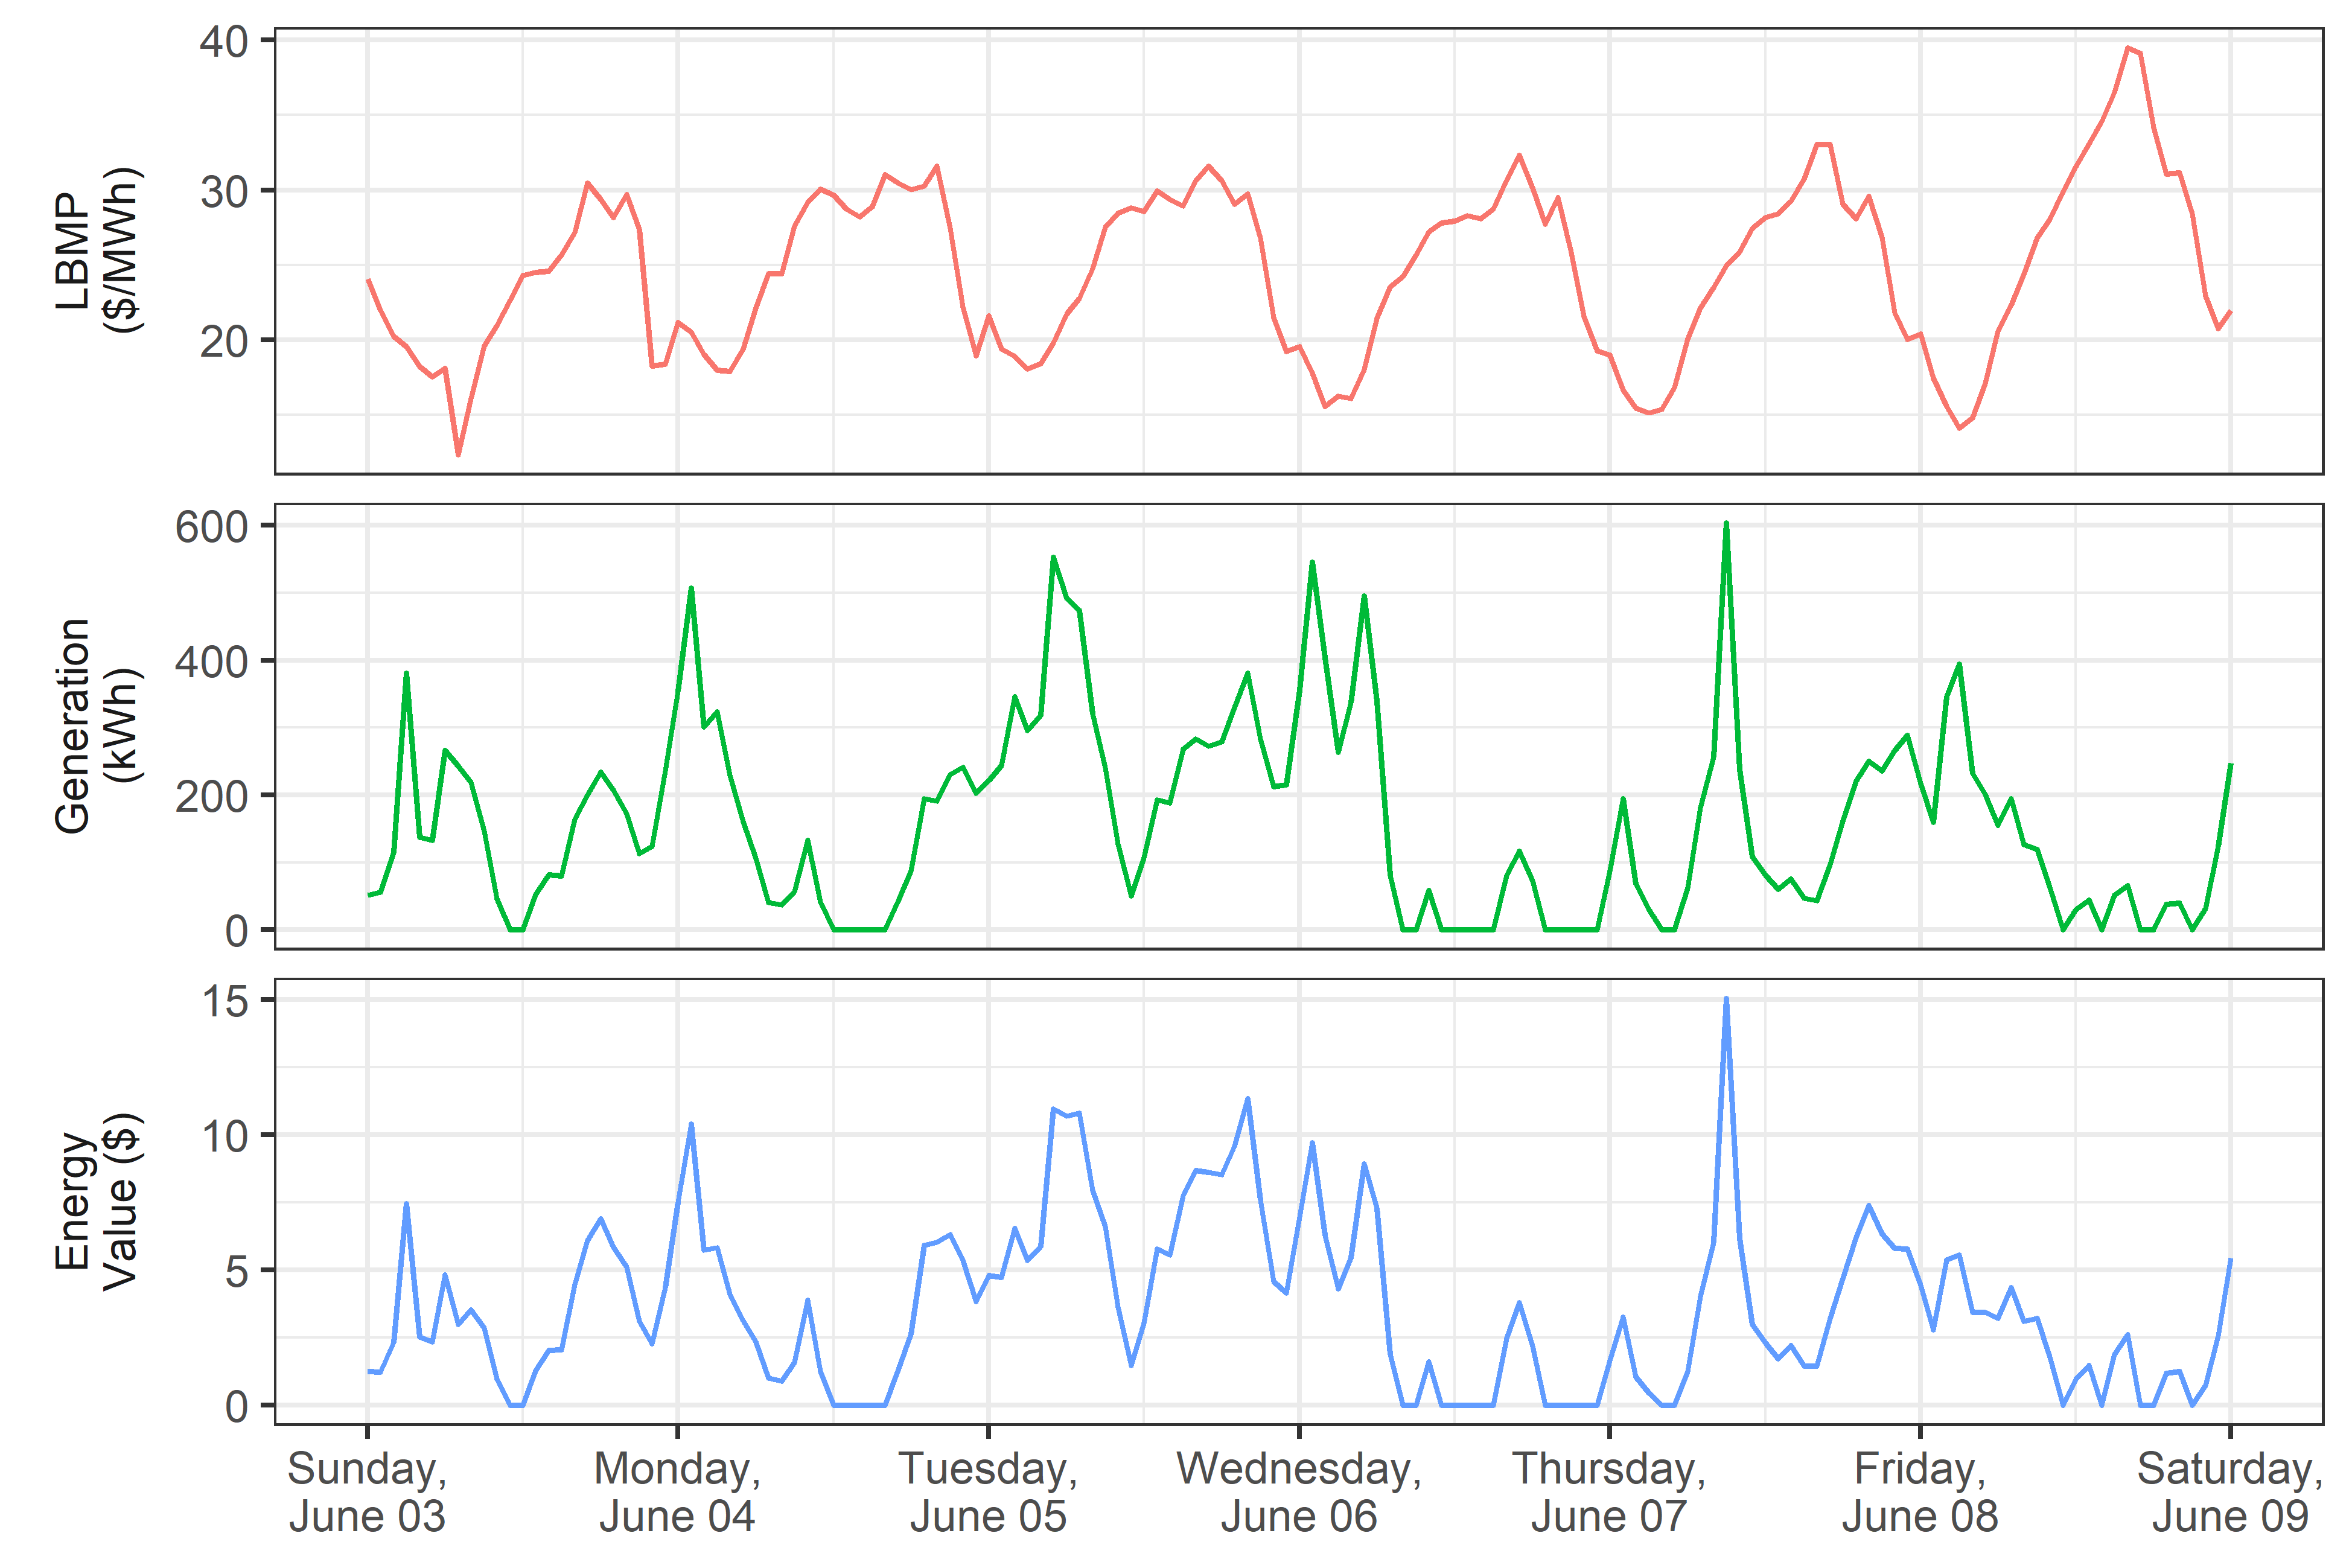
\includegraphics[width=\linewidth]{energy_calc_exp.png}
	  \caption{Example of Calculation of the \aev{} for a Representative Week in June for a Generator in the Hudson Valley NYISO Load Zone.}
	  \label{fig:expaevplot}
\end{conditionalfigure}

%\begin{table}[H]
%\centering
%\begin{tabular}{lcccccccccc}
\toprule
          Name &   Min &  25th &  Median &  Mean &  75th &    Max \\
\midrule
       Capital & 11.07 & 25.13 &   31.48 & 37.80 & 40.14 & 315.24 \\
       Central &  5.99 & 20.76 &   27.12 & 31.01 & 35.32 & 288.17 \\
     Dunwoodie & 11.24 & 24.94 &   31.67 & 37.46 & 40.27 & 313.01 \\
       Genesee &  5.15 & 20.09 &   26.23 & 29.88 & 34.23 & 277.48 \\
 Hudson Valley & 11.18 & 24.76 &   31.35 & 36.92 & 39.78 & 314.17 \\
   Long Island & 12.23 & 29.48 &   37.86 & 45.61 & 48.82 & 303.07 \\
      Millwood & 11.22 & 24.93 &   31.57 & 37.22 & 40.09 & 314.75 \\
 Mohawk Valley &  6.02 & 20.70 &   26.78 & 31.05 & 35.25 & 300.31 \\
        N.Y.C. & 11.37 & 26.30 &   34.20 & 39.93 & 42.49 & 314.74 \\
         North & -2.91 & 14.83 &   20.22 & 24.29 & 29.28 & 281.24 \\
          West &  5.97 & 20.47 &   26.99 & 32.37 & 36.28 & 283.84 \\
\bottomrule
\end{tabular}

%\caption{Summary Statistics for 2018 New York Independent System Operator Day Ahead Market Prices by Zone}
%\label{table:quantlbmpdam}
%\end{table}

% ~~~~~~~~~~~~~~~~~~~~~~~~~~~~~~~~~~~~~~~~ /
%  Generating Capacity Value
% ~~~~~~~~~~~~~~~~~~~~~~~~~~~~~~~~~~~~~~~~ /

\subsubsection{Avoided Capacity Investment Value}
\label{meth_val_aciv}
The \aciv{} value broadly represents the costs avoided for utilities when DER can be reliably expected to help meet peak demand (which drives capacity needs), thereby reducing the capacity the utility must procure either by building their own generation capacity, or by procuring it from a capacity auction. Most of a customer’s electricity bill, and therefore the utility's revenue recovery, is covered by a volumetric energy charge that varies with the consumption of power from the grid. However, many of the costs associated with providing a customer with power are fixed and depend on the customer's (or the power sytem's) instantaneous maximum demand (kW), rather than their total consumption (kWh). This is because a majority of the investments in the power system, from transmission and distribution lines to generating capacity must be sized in order to meet maximum demand. Thus a relatively small number of hours ultimately determine the fixed costs utilities must recover throughout a given year, and even longer as many power system investments have lifespans of several decades. Such fixed costs include, among others, the capital expenditures (CAPEX) required to build a new generating unit and the fixed operating and maintenance costs (FOM) associated with operating the unit. 

As New York is a deregulated energy market, the utilities procure generating capacity to meet their peak demand through capacity auctions, as opposed to building and operating the plants themselves. Accordingly, this analysis looks at the reduction in these capacity auction procurement requirements enabled by DER exports to determine the \aciv{}. Generating capacity needs and capacity auction requirements are determined by the utilities by examining their forecasted highest periods of demand which occur in a small number of hours per year. As it is these select number of hours that contribute to peak demand and determine capacity auction requirements, only DER exports within these hours can actually provide capacity value by reducing utility purchases from the capacity market. This  is accounted for in the VDER framework and this analysis by only allowing exports during certain hours to qualify for the \aciv{}, defined as hours during which the entire NYISO territory is likely to experience peak demand. These hours are defined in the latest Value Stack Order as non-holiday weekdays from June 25\textsuperscript{th} to August 31\textsuperscript{st} for the hours between 2:00 PM and 6:00 PM, inclusive. Figure \ref{fig:capvalheatmap} below shows the valid hours during which DER exports could earn a capacity value for a typical week in July. Exports during these hours qualify for a value that is determined by the capacity auction for the NYISO load zone from which the DER is exporting.

\begin{conditionalfigure}[!htb]
  \centering
	  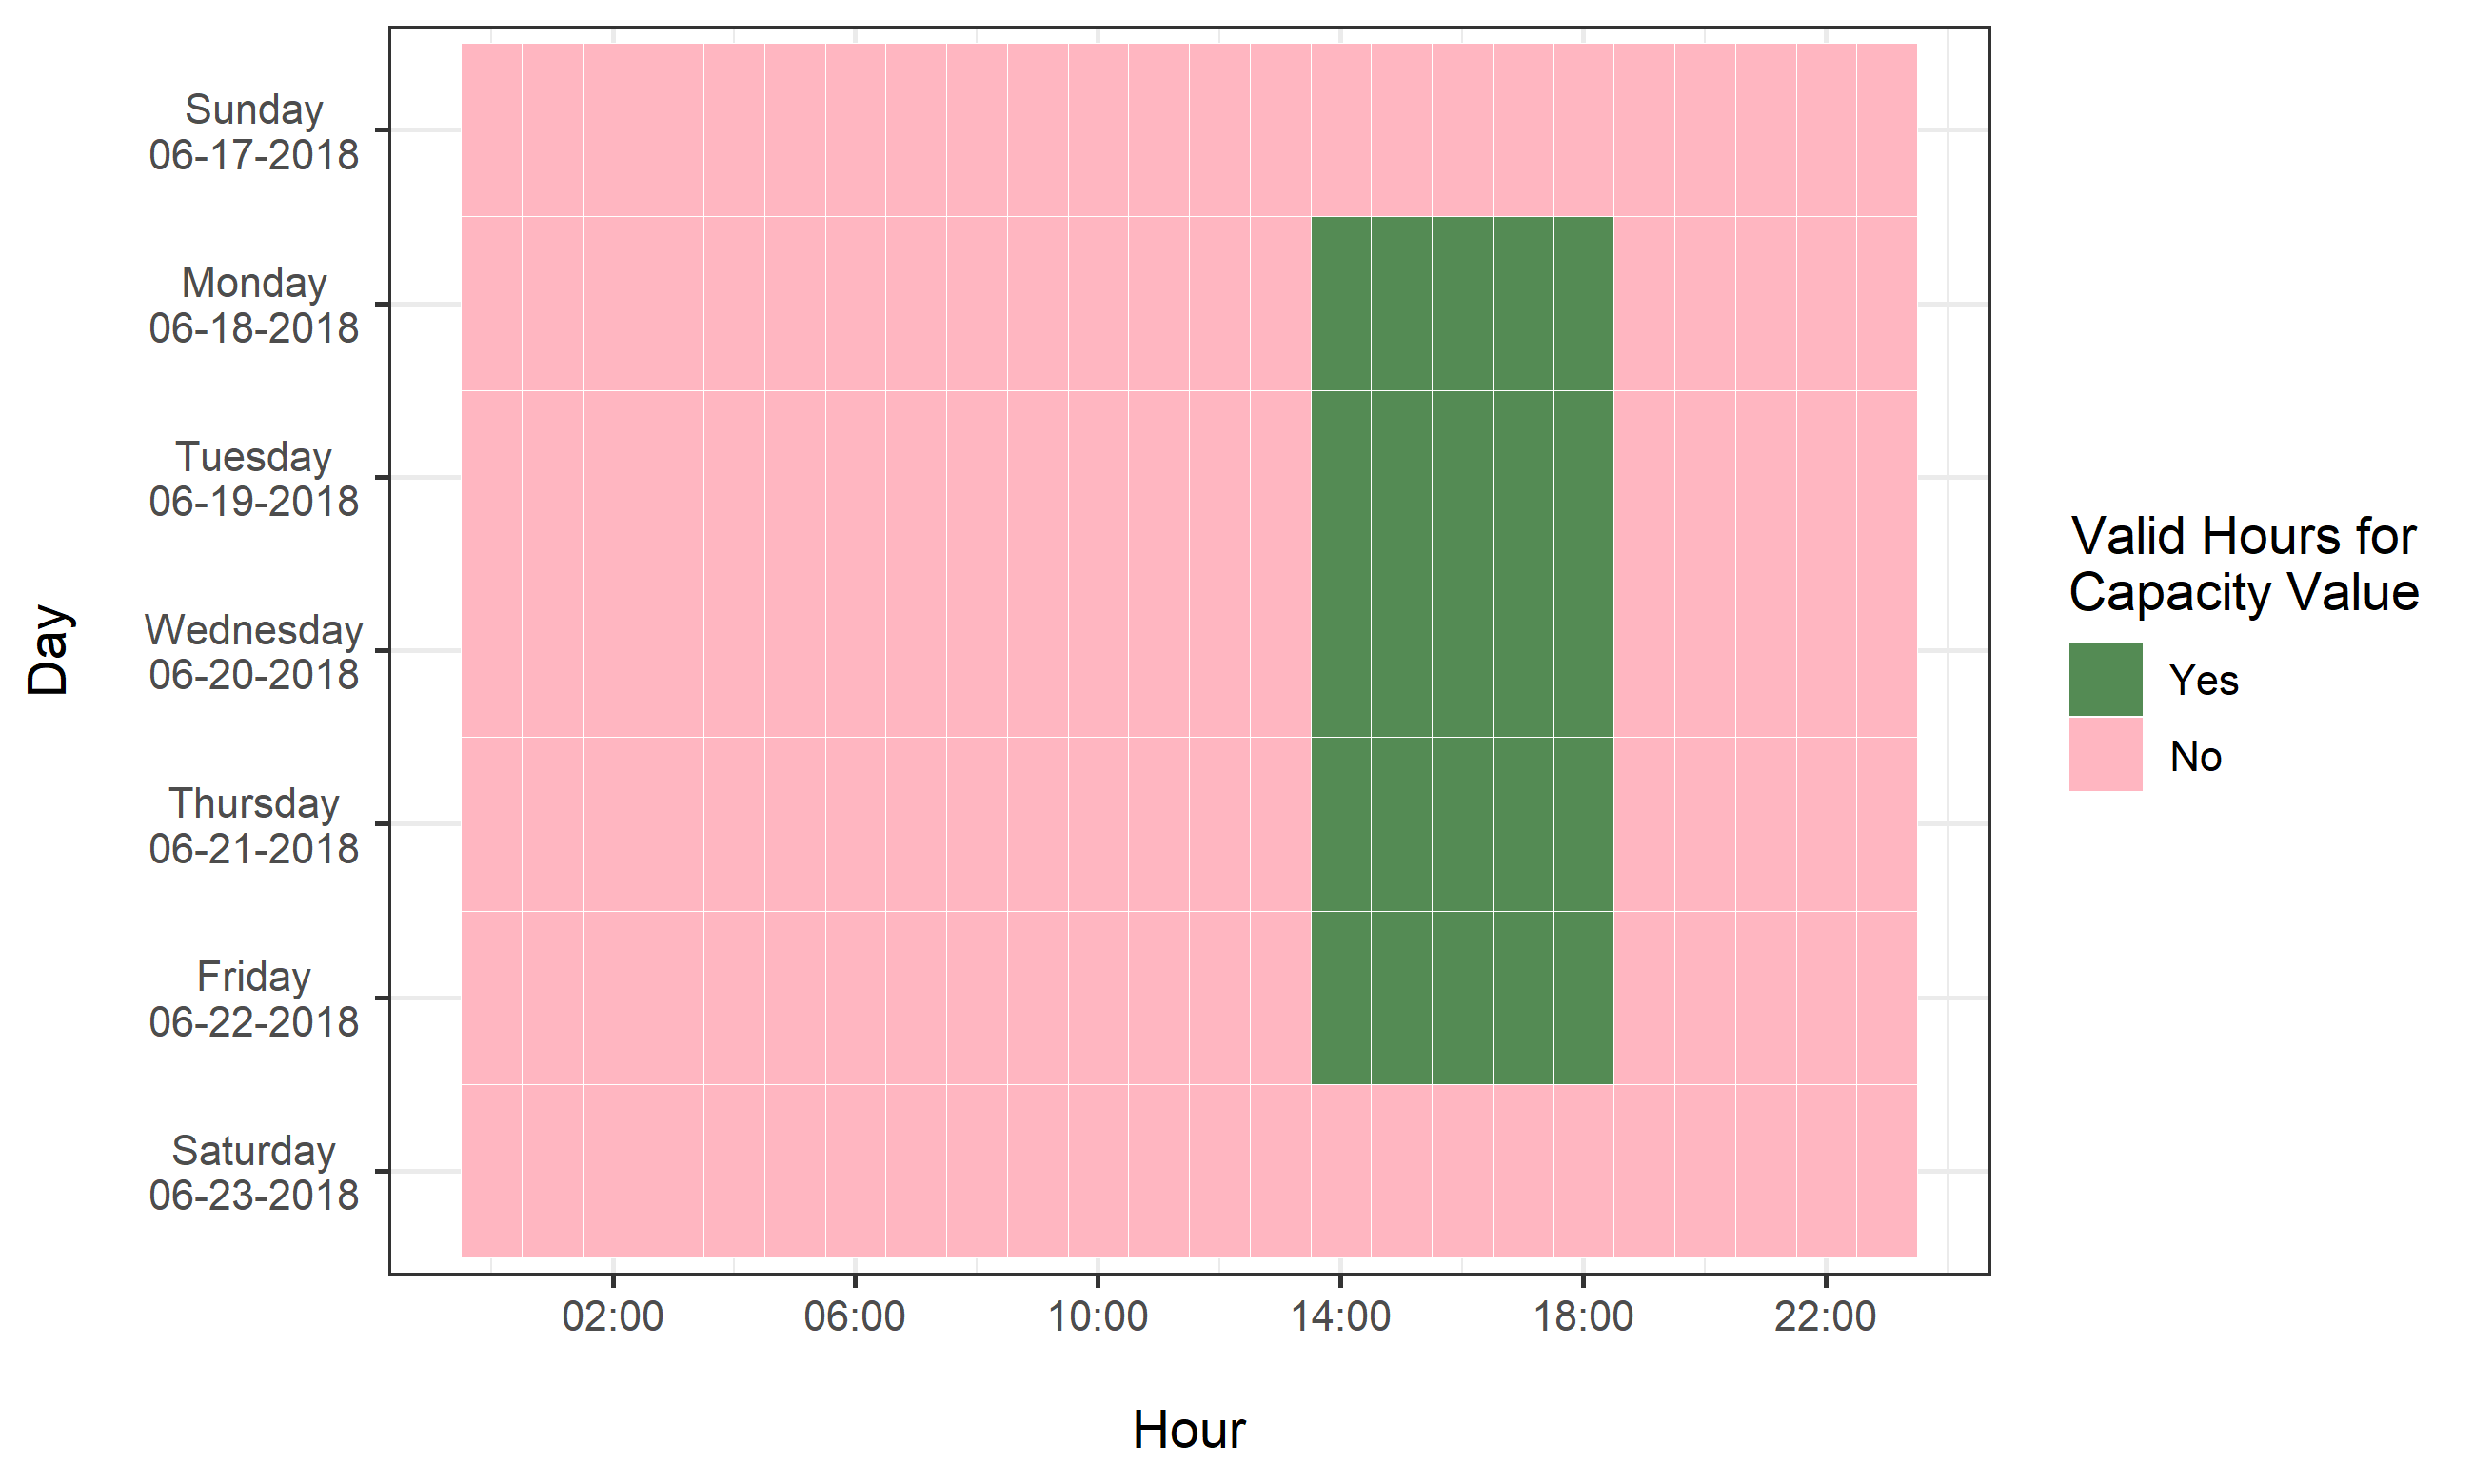
\includegraphics[width=\linewidth]{cap_val_hours.png}
	  \caption{Valid Hours for DER Exports to Earn Capacity Value. Source: \citet{nypsc_matter_2019}.}
	  \label{fig:capvalheatmap}
\end{conditionalfigure}

% Latest Value Stack Order available here: https://www.nyserda.ny.gov/-/media/NYSun/files/Updated-Value-Stack-Order-2019-04-18.pdf

\vspace*{10mm}
\begin{centering}
\large\textsc{which method is this in the vder stack \ldots}
\end{centering}
\vspace*{10mm}

The specific value is calculated by taking the sum of the monthly capacity auction results (in \$/kW-month) for an entire year (which yields \$/kW-year), measured from May 31\textsuperscript{st} to May 31\textsuperscript{st}. The monthly capacity auction results can be accessed at \cite{nyiso_monthly_2020}. This annual capacity auction total (\$/kW-year) is divided by the number of qualifying hours in that year (from June 25\textsuperscript{th} to August 31\textsuperscript{st} on non-holiday weekdays from 2:00 PM to 6:00 PM), either 240 hours or 245 hours depending on whether Independence Day falls on a weekday during the year, to yield a capacity value in \$/kWh \cite{nypsc_matter_2019}. This value is expressed for each zone for three years from 2016 to 2018 in Table \ref{table:icapprices} and is shown graphically for the year \hl{2018} in Figure \ref{fig:chloroicap}. This value is then applied to all exports to the grid from the DER which occur in the valid hour window to calculate the \aciv{}. 

%As with the \aev{}, these values are then scaled up by the associated utility transmission and distribution losses, as generation used to meet demand closer to load experiences little losses, relative to transmission-sited generation (see \atdlv{}).

%Equation \eqref{eq:2} mathematically expresses how the \aciv{} is determined for a generator \textit{i} located in NYISO load zone \textit{j}.
%\begin{equation}
%Value_{Capacity} (i) = \sum_{\substack{t=0 \\i\;\subseteq\;j \\t\;\subseteq\;valid\;hours}}^{n=240\;or\;245} \underbrace{Export_{DER} (i,t)}_\text{FOM wind generation} \cdot \underbrace{Capacity\;Price_{DAM}(j)}_\text{ICAP Auction Price} \label{eq:2}
%\end{equation}

\begin{conditionaltable}[!htb]
\centering
    \pgfplotstabletypeset[column type = lccc, multicolumn names,
      col sep=comma,
	display columns/0/.style={string type, column name=Zone},
	display columns/1/.style={fixed, fixed zerofill, precision = 3, column name=2016},
	display columns/2/.style={fixed, fixed zerofill, precision = 3, column name=2017},
	display columns/3/.style={fixed, fixed zerofill, precision = 3, column name=2018},
	every head row/.style={
		before row={\toprule}, 
		after row= & \$/kWh & \$/kWh & \$/kWh\\
					\midrule
		},
	every last row/.style={
		after row=\bottomrule
		},
    ]{\icapdata}
\caption{Historical Normalized Capacity Auction Prices. Data Source: \citet{nyserda_solar_2019}.}
\label{table:icapprices}
\end{conditionaltable}

\begin{conditionalfigure}[!htb]
  \centering
	  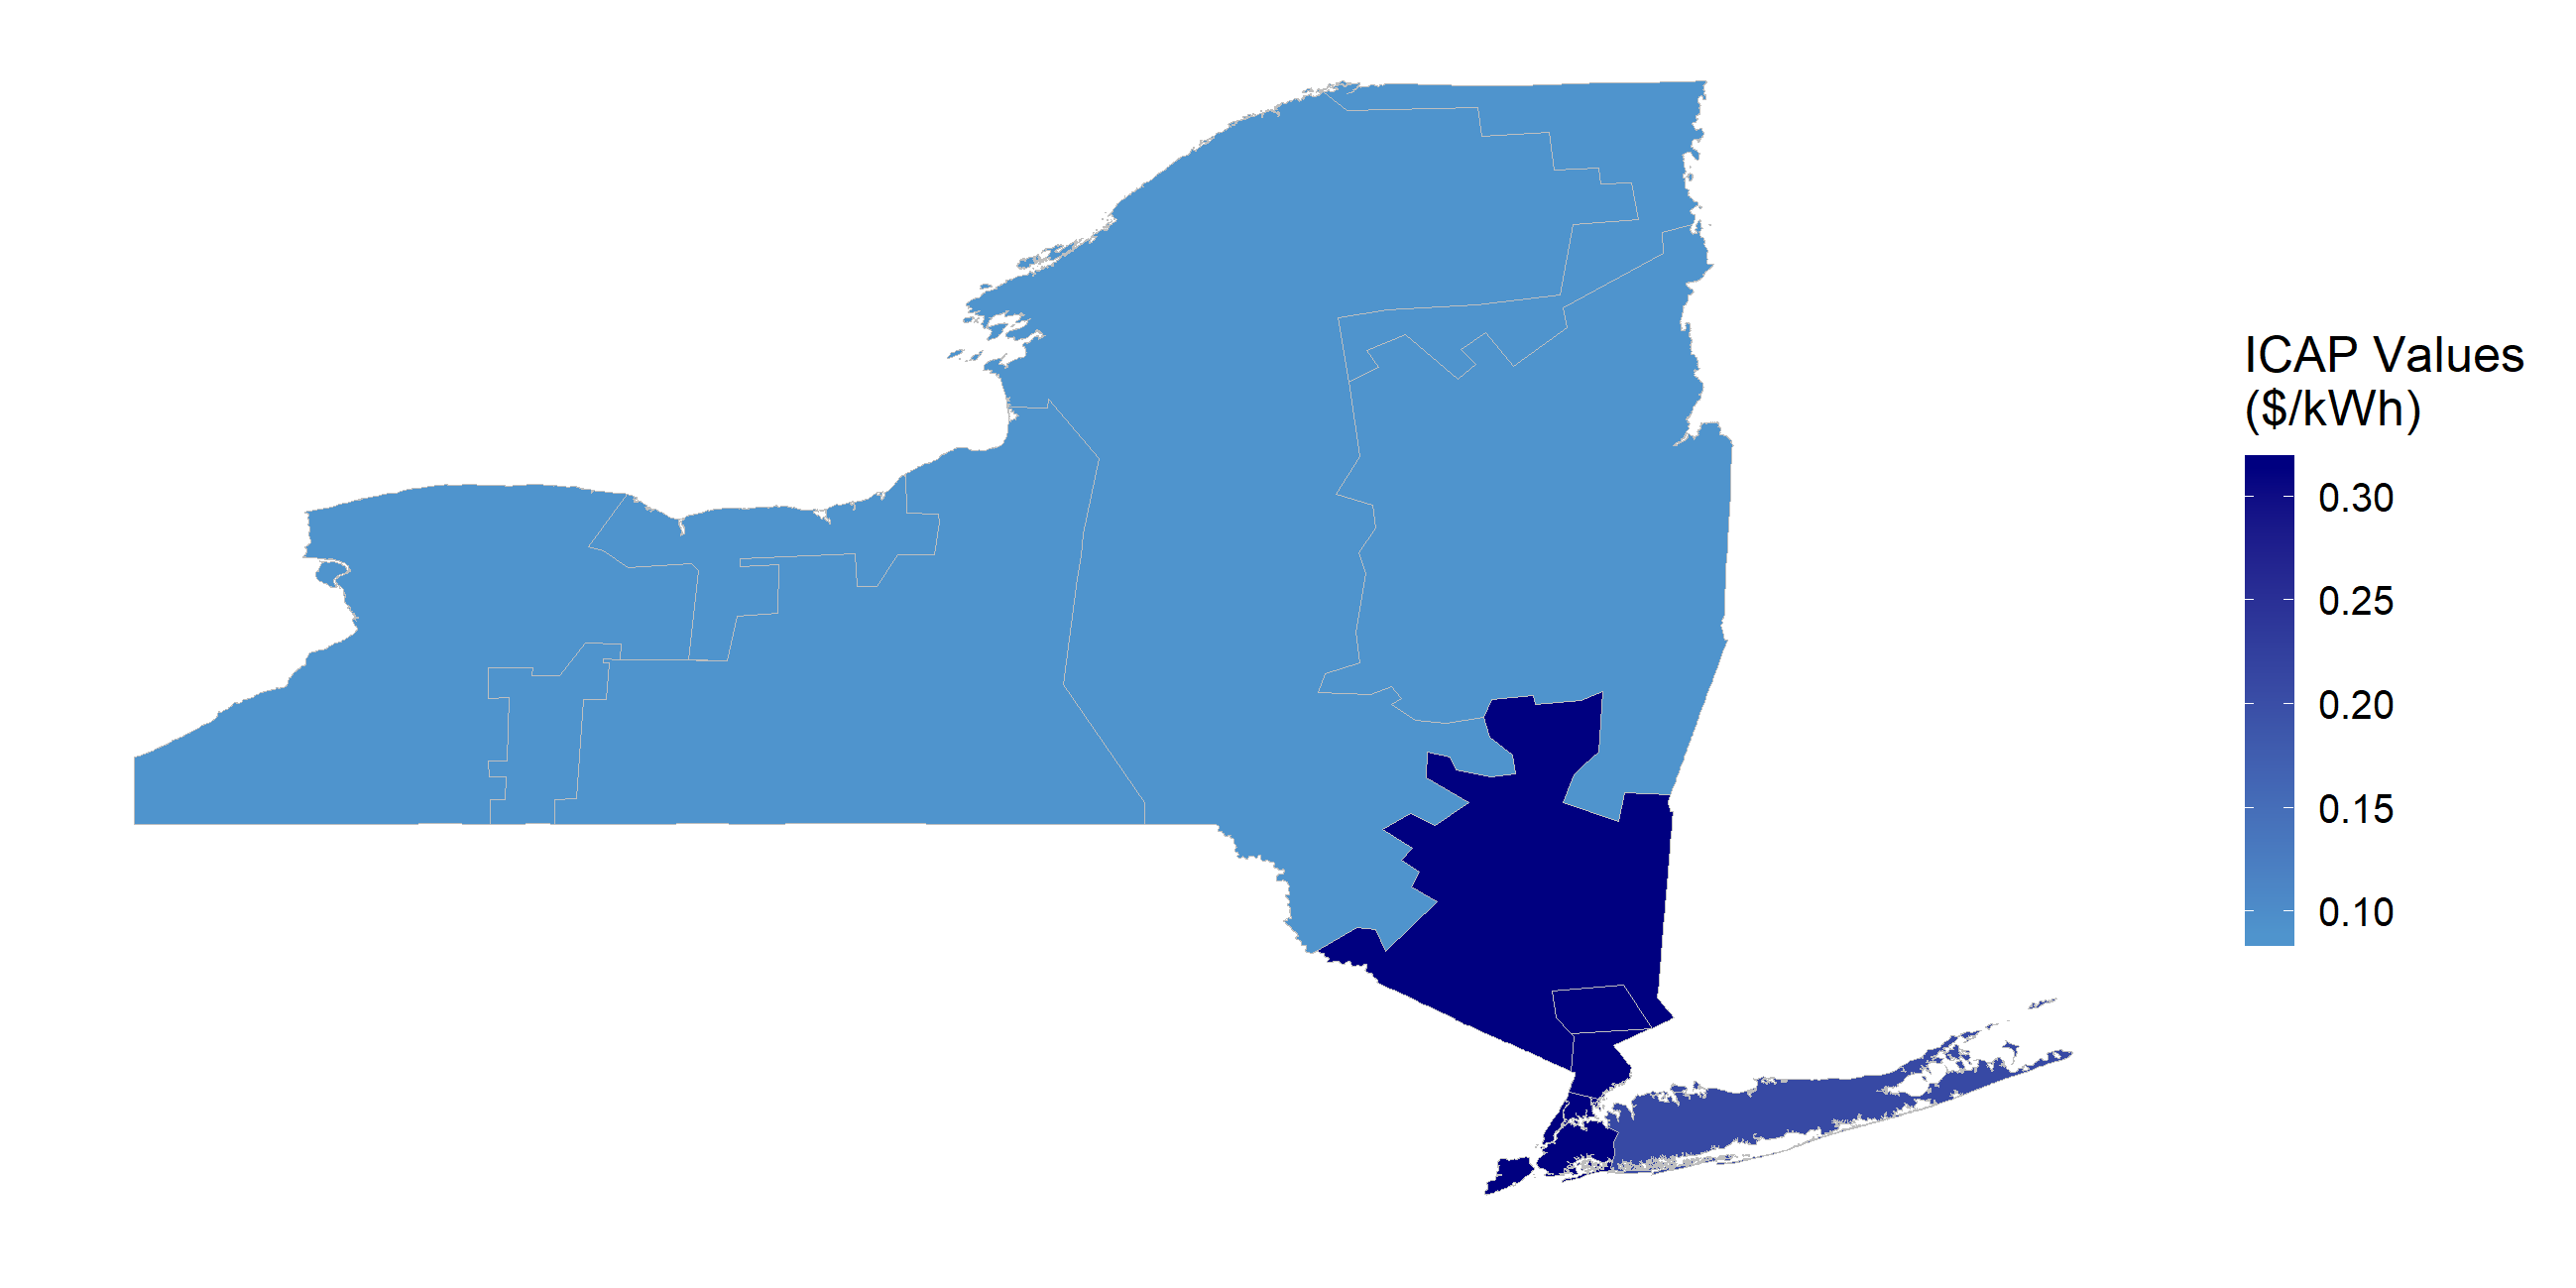
\includegraphics[width=\linewidth]{ICAP_chloropleth.png}
	  \caption{Chloropleth of ICAP Values by NYISO Load Zone. Data Source: \citet{nyserda_solar_2019}}
	  \label{fig:chloroicap}
\end{conditionalfigure}

% ~~~~~~~~~~~~~~~~~~~~~~~~~~~~~~~~~~~~~~~~ /
%  DRV
% ~~~~~~~~~~~~~~~~~~~~~~~~~~~~~~~~~~~~~~~~ /

\subsubsection{Demand Reduction Value}
\label{meth_val_drv}

Similar to the \aciv{}, the \drv{} is a measure of the ability of DER exports to reduce the overall infrastructure a utility must invest in, by reducing the load that utility must meet during peak periods. Rather than addressing the fixed costs associated with the generation fleet, however, the \drv{} expresses the value of reducing fixed costs associated with the transmission and distribution capacity needed to deliver power to customers. The infrastructure and associated costs for delivering power to customers varies strongly between and even within utilitiy territories and unlike \hl{generating capacity, there is no central auction for distribution and transmission capacity as this capacity cannot redistributed once built}. 

Accordingly, both the valid hours during which DER exports qualify for the \drv{} as well as the monetary value associated with exports are utility-specific.  For this analysis, the utility-specific valid hours and monetary value were taken directly from the Value Stack Order. \hl{The specific monetary value for exports is determined by each utility as part of its Marginal Cost of Service (MCoS) Study, although the methodology is set to be made more transparent and unified at a future date}. Table \ref{table:drvinfo} shows the relevant terms for the DRV calculation for each utility: the annual DRV value as well as the valid hours and dates for earning the DRV. % available here: https://www.nyserda.ny.gov/-/media/NYSun/files/Updated-Value-Stack-Order-2019-04-18.pdf

The monetary value for the \drv{} is given in terms of a fixed, 10-year \$/kW-year rate. This value is converted to \$/kWh by dividing ten times the annual value by the number of qualifying hours in that 10-year fixed term. Unlike the \aev{} and \aciv{}, the \drv{} monetary value is set at a fixed rate for a 10 year period, rather than fluctuating month to month or hour to hour as with the day-ahead and capacity auction markets. The monetary value was fixed to help ensure a level of investor certainty for customers and renewable energy developers. As these projects require significant upfront capital to develop, investors must be certain than they can recuperate their sunk capital expenditures through revenues earned throughout the projects life. When this revenue fluctuates with energy and capacity markets, it better represents that distributed system's contribution to the power system, but it can be difficult to ensure cost recovery and may deter investment.  

%Equation \eqref{eq:3} mathematically expresses how the \drv{} is determined for a generator \textit{i} located in utility territory \textit{k}.

For Consolidated Edison, ConEd, rather than have a fixed DRV window for its entire territory, the utility divided its territory into four different, non-contiguous subsections based on each subsection's summer peak. Exports in each of these sections are awarded at the same value, but only qualify in different hours during the same June 24\textsuperscript{th} to September 15\textsuperscript{th} window. These subsections are reflected in Table~\ref{table:drvinfo} as well as in Figure~\ref{fig:drvconed}. \hl{The subsections of the utility were determined by carefully comparing utility pdf maps of the subsections in their territory against publicly available maps of the various boroughs and neighborhoods in the Consolidated Edison territory} \cite{consolidated_edison_con_2019}. \textcolor{pink}{\textsc{source-Margaret}}.\footnote{The utility maps actually display the Commercial System Relief Program (CSRP) areas in their territory, which were also used when creating the DRV subsections in their territory \cite{nypsc_matter_2019}.}

\begin{equation}
Value_{Demand Reduction} (i) = \sum_{\substack{t=0 \\i\;\subseteq\;k \\t\;\subseteq\;valid\;hours}}^{n} \underbrace{Export_{DER} (i,t)}_\text{FOM wind generation} \cdot \frac{\overbrace{DRV\;Price (k)}^\text{Utility DRV \$ value} \cdot 10}{\underbrace{n_{\:valid\:hours}}_\text{number of valid hours in 10 year period}} \label{eq:3}
\end{equation}

\begin{conditionaltable}[!htb]
\centering
    \pgfplotstabletypeset[column type = lcrlc, multicolumn names,
      col sep=comma,
	display columns/0/.style={string type, column name=Utility},
	display columns/1/.style={string type, column name= Annual Value},
	display columns/2/.style={string type, column name= Hour Window},
	display columns/3/.style={string type, column name= Date Window},
	display columns/4/.style={fixed, fixed zerofill, precision = 3, column name= DRV Value},
	every head row/.style={
		before row={\toprule}, 
		after row= & \$/kW-year & non-holiday & weekend hours & \$/kWh\\ 
					\midrule
		},
	every last row/.style={
		after row=\bottomrule
		},
    ]{\drvvals}
\caption{DRV Values and Time Windows for NY Utilities.\\\hspace{\textwidth} *:Consolidated Edison, or ConEd, chose to divide its utility territory into four different, non-contiguous subsections based on each subsection's summer peak. Exports in each of these sections are awarded at the same value, but only qualify in different hours during the same June 24\textsuperscript{th} to September 15\textsuperscript{th} window.\\\hspace{\textwidth} **: New York State Electricity and Gas utility has two distinct peaks in its territory, one in the summer and one in the winter. In order to incentivize exports to reduce both peaks, the utility offers a DRV bonus in the summer and winter. \$/kWh values are still calculated by dividing ten times the annual amount by the number of qualifying hours over a ten-year period. Source: \citet{nypsc_matter_2019}.}
\label{table:drvinfo}
\end{conditionaltable}

\begin{conditionalfigure}[!htb]
  \centering
	  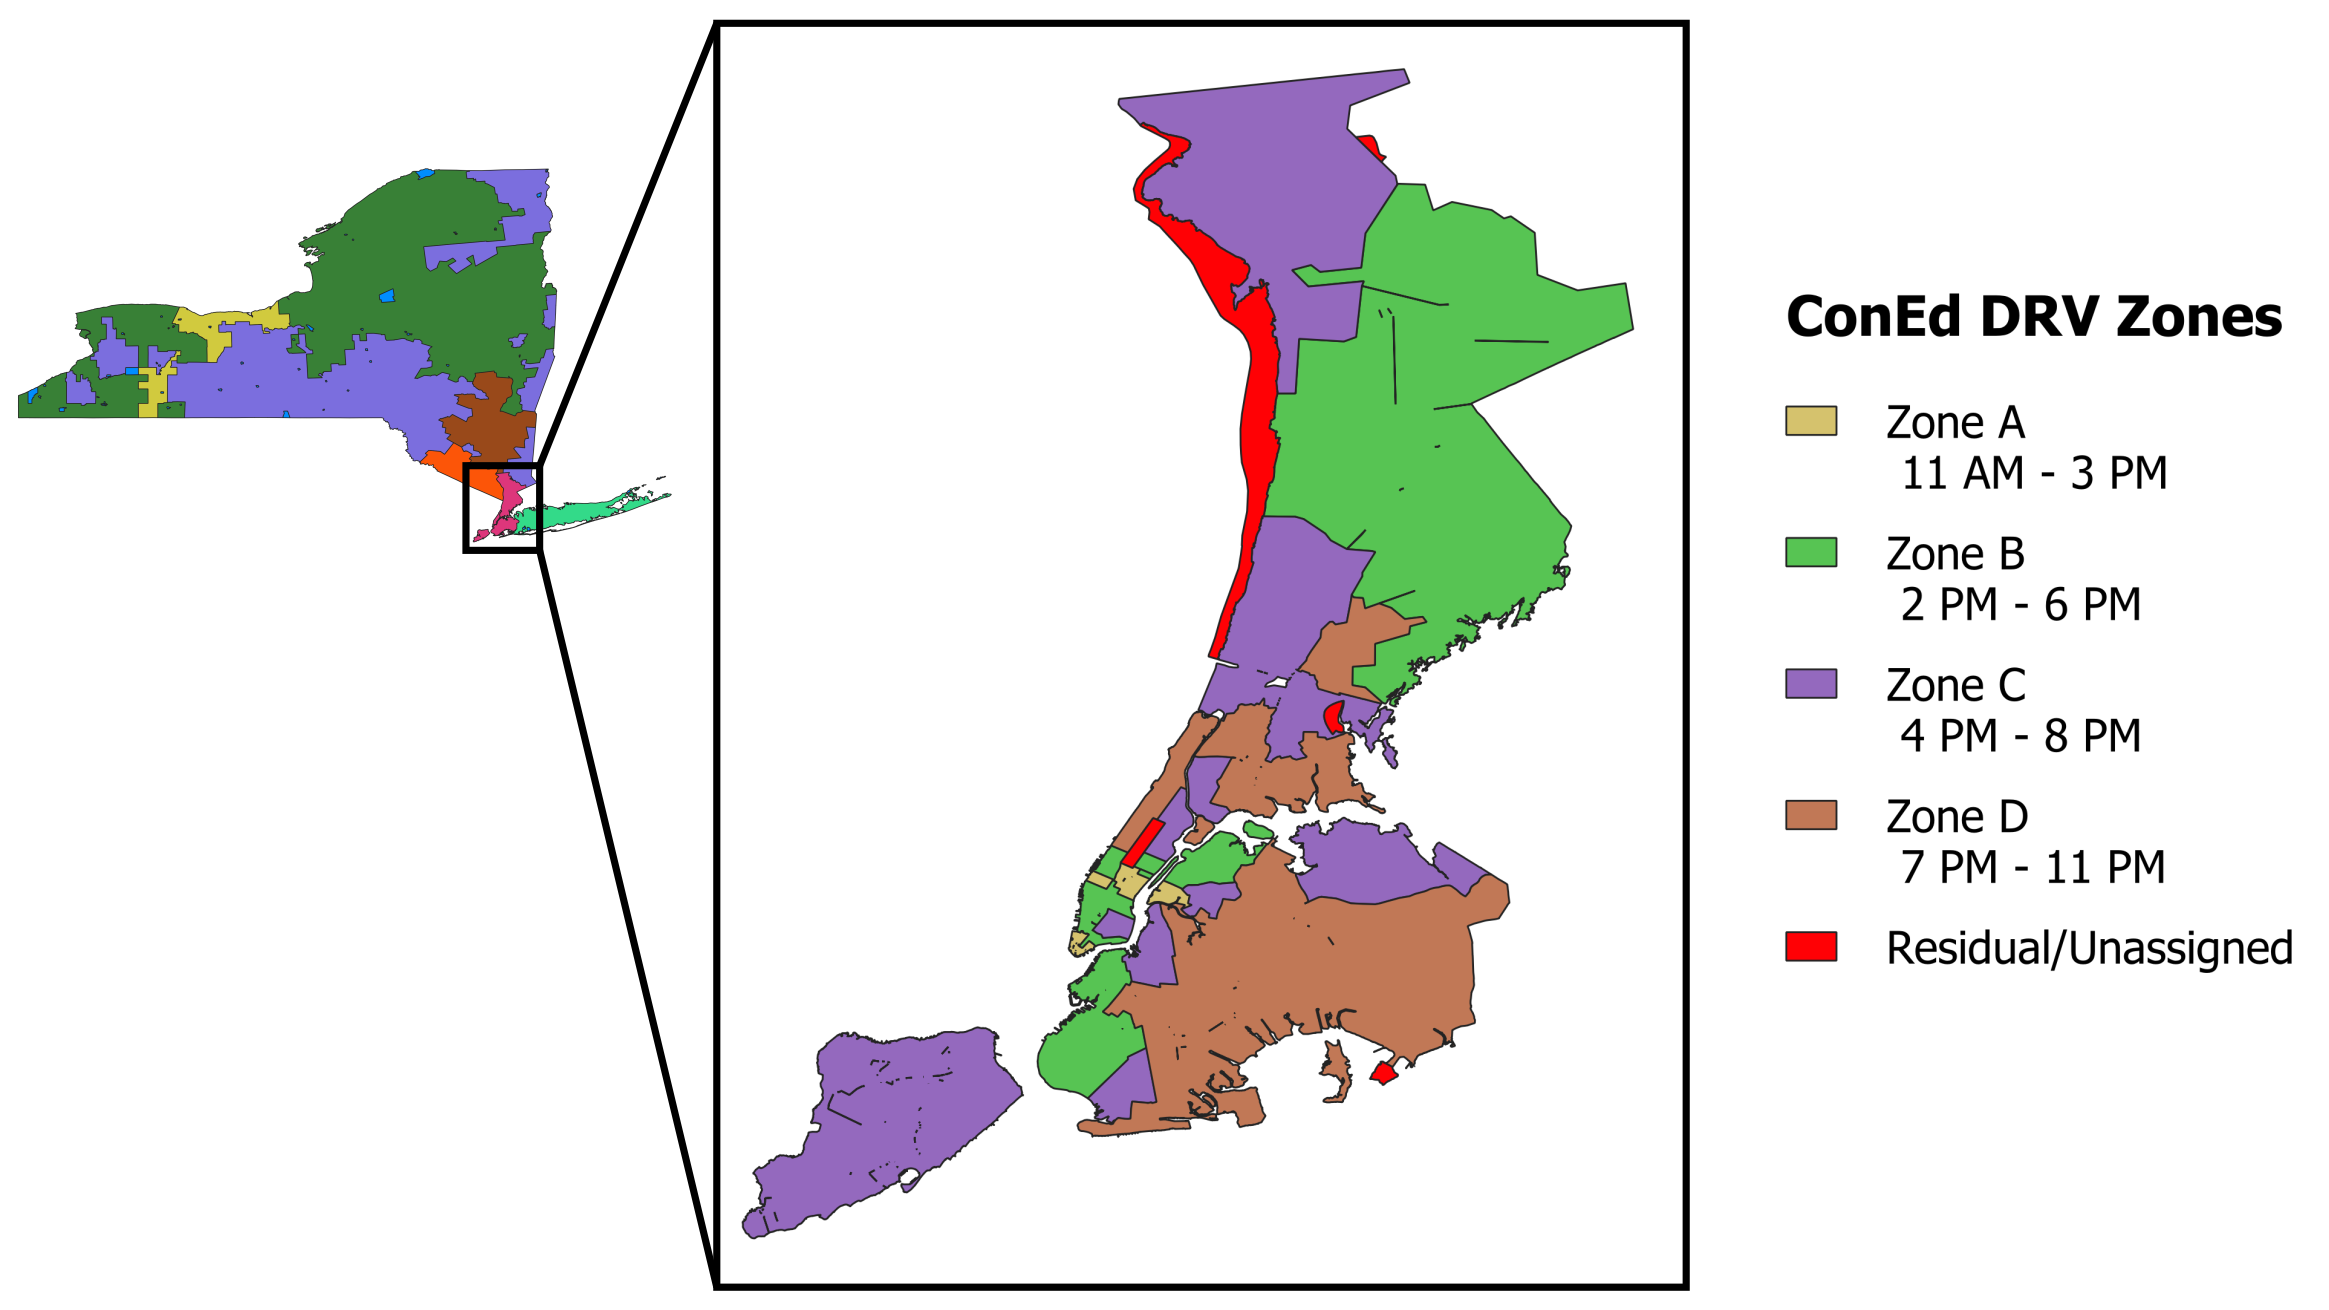
\includegraphics[width=\linewidth]{ConEd_DRV_Zones_edited.png}
	  \caption{The DRV Subsections of the Consolidated Edison Utility Territory. Source: \textcolor{pink}{\textsc{source-Margaret}}}
	  \label{fig:drvconed}
\end{conditionalfigure}

\hl{map zoomed in of ConEdison DRV zones}

% ~~~~~~~~~~~~~~~~~~~~~~~~~~~~~~~~~~~~~~~~ /
%  LSRV
% ~~~~~~~~~~~~~~~~~~~~~~~~~~~~~~~~~~~~~~~~ /

\subsubsection{Locational System Relief Value}
\label{meth_val_lsrv}

The \lsrv{} measures the value of a DER's export to reduce congestion at specific points within the power system by injecting power near demand. This value is limited not only to injections within specific time periods, but also to specific subsections of the power system. Utilities have identified portions of their territory that experience significant congestion during their territory's peak period that could benefit from more local generation. Only exports originating from within these `LSRV zones' can qualify for LSRV compensation. Figure \ref{fig:lsrvzoneexp} highlights an example of an LSRV zone in the Long Island Power Authority Territory.

\begin{conditionalfigure}[!htb]
  \centering
	  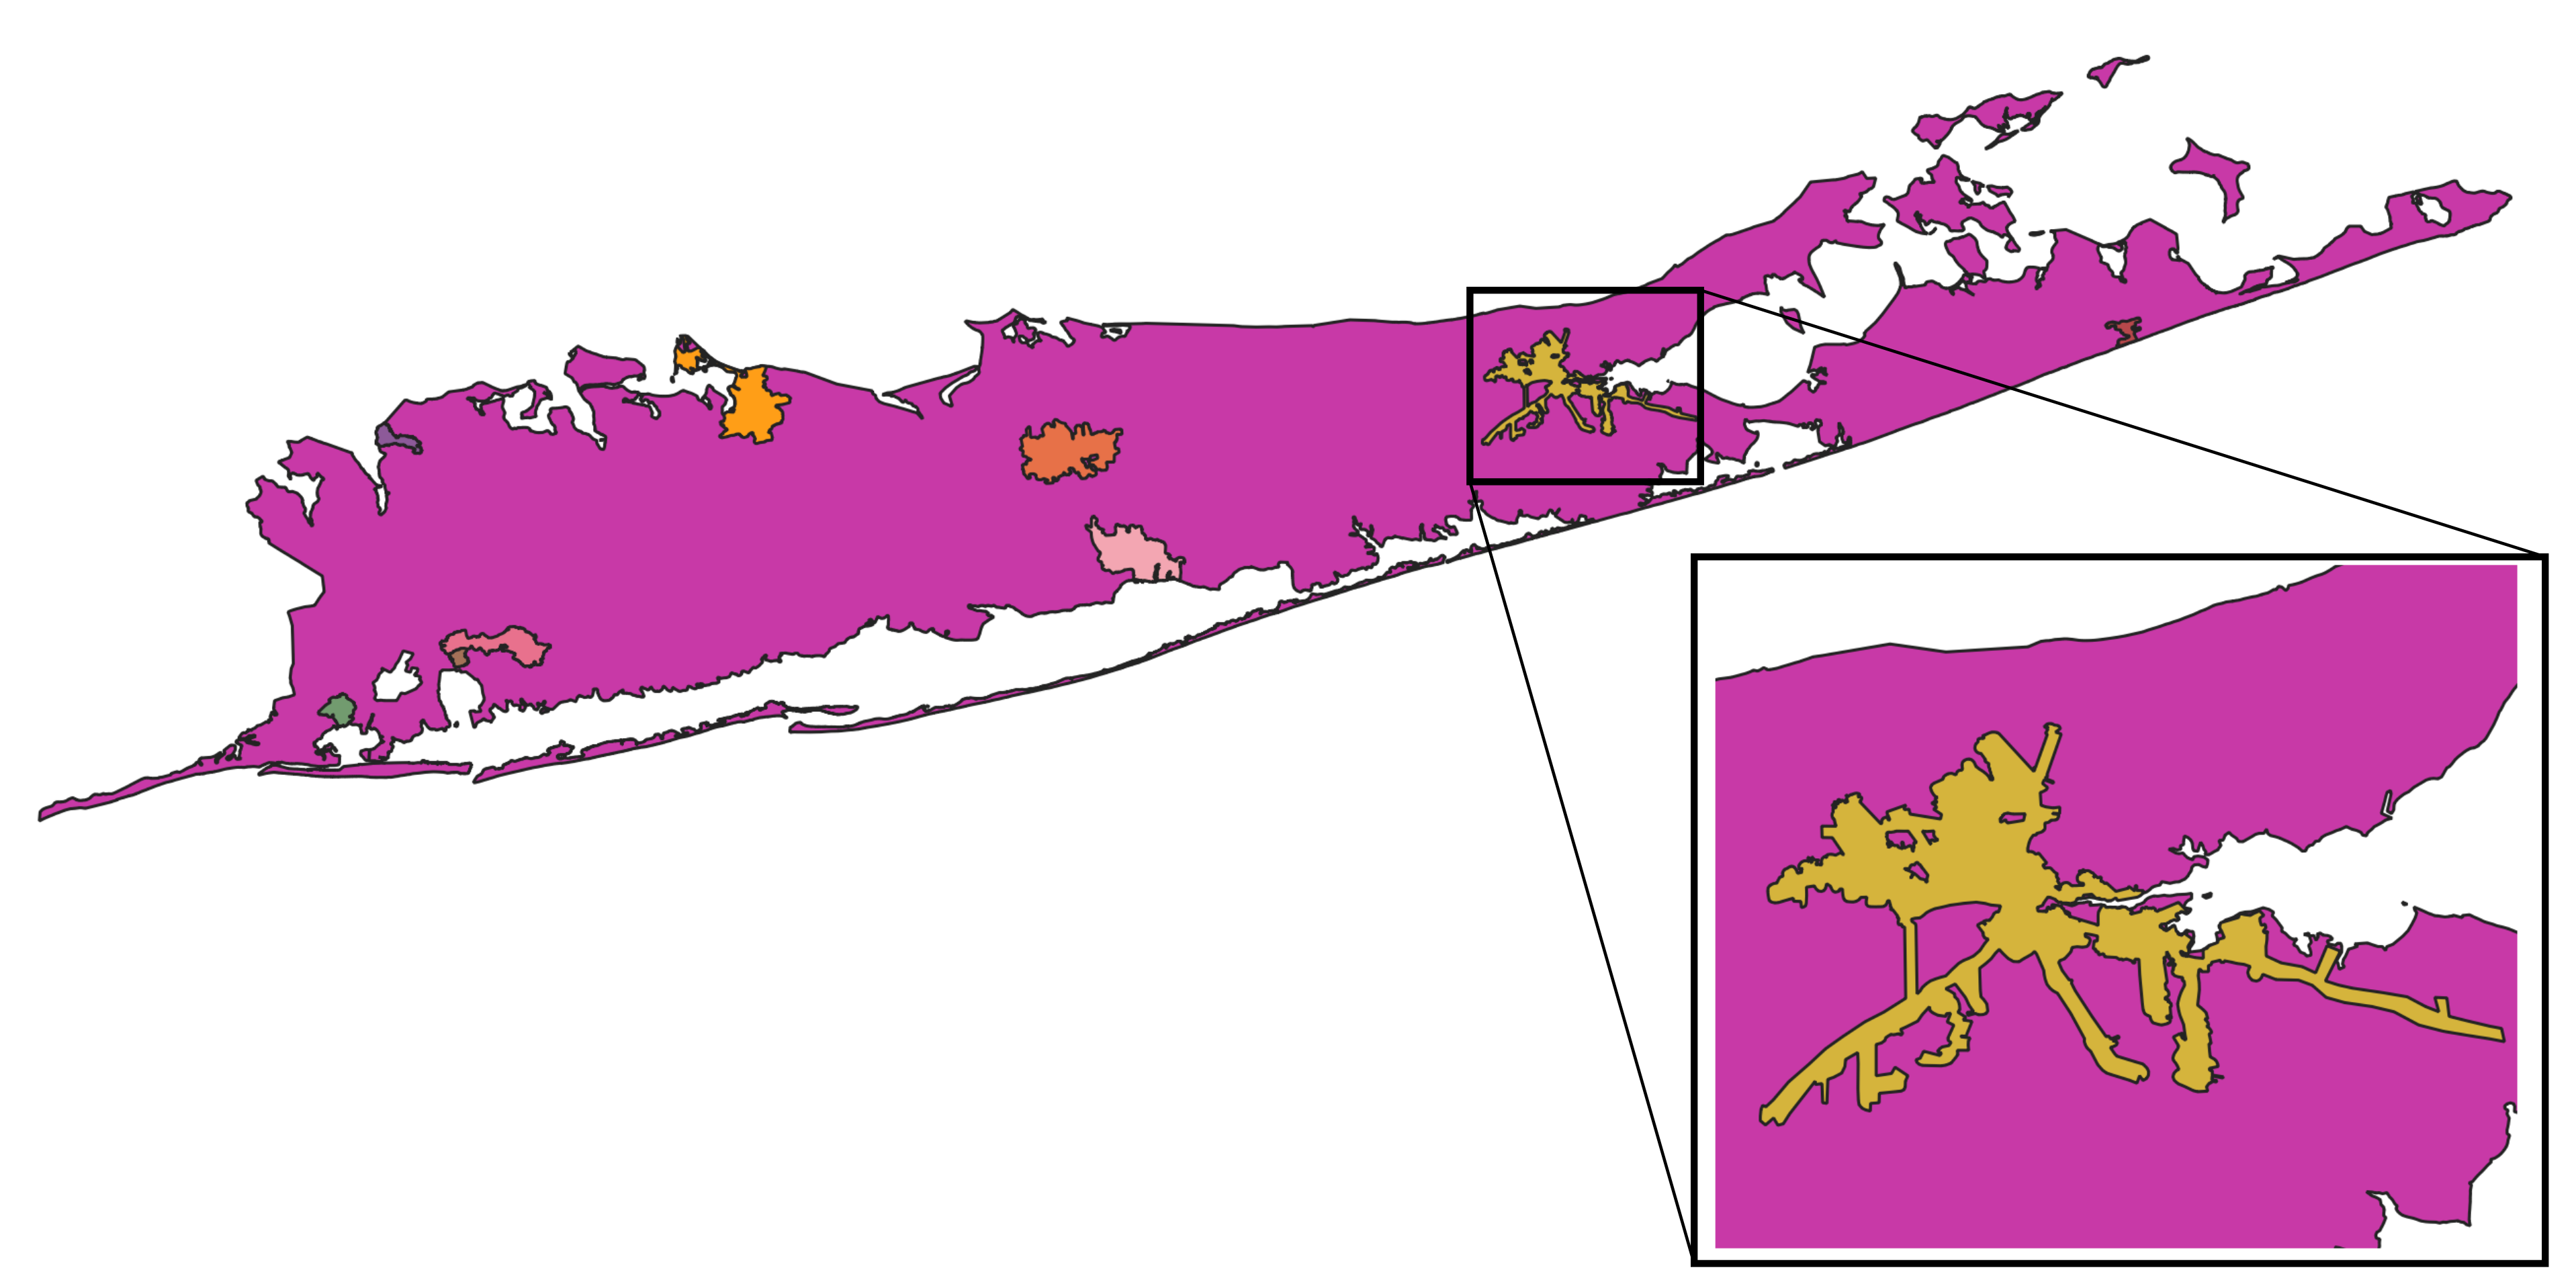
\includegraphics[width=\linewidth]{LSRV_Zone_Closeup_cropped.png}
	  \caption{Long Island Power Authority LSRV Zones with focus on Specific Zone.}
	  \label{fig:lsrvzoneexp}
\end{conditionalfigure}

Unlike the DRV or \aciv{}, the time periods during which exports qualify are determined dynamically by the utilities themselves through `calls'. Utilities must alert generators of such calls twenty-one hours in advance of the actual call. Utilities are required to make at least 10 calls per year and each call must be at least 1 hour in duration and no more than 4 hours in duration. As a default the hours, during which a call could be made are the same hours for the DRV value, however, utilities have the option of setting separate/unique LSRV hours distinct form the DRV window based on `sub-system peaks'.  Table \ref{table:lsrvinfo} shows the the annual LSRV value, where the the valid hours and dates for earning the LSRV are assumed to be the same as the DRV. The LSRV Value (\$/kW-call) is derived based on the minimum 10 calls/year quota set by the NYPSC. Although a minimum of 10 calls must be made per year, it is possible for the utility to make additional calls, which means that generators could theoretically earn more than the annual LSRV value.

\begin{conditionaltable}[!htb]
\centering
    \pgfplotstabletypeset[column type = lcc, multicolumn names,
      col sep=comma,
	display columns/0/.style={string type, column name=Utility},
	display columns/1/.style={string type, column name= Annual Value},
	display columns/2/.style={fixed, fixed zerofill, precision = 3, column name= LSRV Value},
	every head row/.style={
		before row={\toprule}, 
		after row= & \$/kW-year & \$/kW-call\\ 
					\midrule
		},
	every last row/.style={
		after row=\bottomrule
		},
    ]{\lsrvvals}
\caption{LSRV Values and Time Windows for NY Utilities}
\label{table:lsrvinfo}
\end{conditionaltable}

Also dissimilar to the DRV, only the minimum instantaneous generation within the given call is applied to the \$4/kw-call value for the duration of the call (e.g. if a generator exported 4 kW, 10 kW, 15 kW and 7 kW within a 4 hour call, the export magnitude used to determine the LSRV value in each hour would be 4 kW and the total LSRV value for that call would be $4kW*Call-value_LSRV$). As with the DRV, the monetary value for the LSRV is given in \$/kW-year and must be converted by dividing by 10 (for each call) yielding \$/kW-call. The monetary value can be unique within each utility territory. %Equation \eqref{eq:4} mathematically expresses how the \lsrv{} is determined for a generator \textit{i} located in utility territory \textit{k} during a call \textit{c} of duration \textit{d}.

%\begin{equation}
%Value_{Locational System Relief} (i) = \sum_{\substack{t=0 \\i\;\subseteq\;k}}^{n} \underbrace{\min_{\forall t \in c} Export_{DER} (i,t)}_\text{FOM wind generation} \cdot \frac{\overbrace{LSRV\;Value (k)}^\text{LSRV \$ value}}{10} \label{eq:4}
%\end{equation}


%$\underbrace{\overbrace{a+b+c}^6\cdot \overbrace{d+e+f}^7}_\text{meaning of life} = 42$

\vspace*{10mm}
\begin{centering}
\textsc{Need to add something about how the LSRV \$ values are actually determined, i.e. explain the Marginal Cost of Service studies and cite ConEd's report by Brattle \ldots}
\end{centering}
\vspace*{10mm}


\subsubsection{Avoided Transmission and Distribution Losses Value}
\label{meth_val_atdlv}

\vspace*{10mm}
\begin{centering}
\textsc{Need to check and see which losses are being applied to which value \& utility territory. It appears that only the energy and capacity value qualify for the scale-up, see the losses and factors of adjustment in the calaculator on the `Losses' sheet \ldots}
\end{centering}
\vspace*{10mm}

When utilities deliver energy from large, centralized generators in order to meet customer demand, that delivery suffers from losses on both the transmission system and distribution system. These losses have a vareity of causes, such as resistive `skin' losses or `corona' losses caused by sufficiently high line-to-line voltages, but in general the longer the distance energy must travel between generating source and the demand sink, the higher the losses the energy will experience. Compared to satisfying demand from centralized generating resources, meeting customer demand with generators located nearby on the distribution system suffers fewer losses. This is particularly true in the case of behind-the-meter systems satisfying onsite customer demand. To account for these reduced losses, the \aev{} and the \aciv{} should be scaled up by the appropriate transmission and distribution (T\&D) losses. This is because less energy is ultimately required from distributed assets than centralized assets to meet demand, while the same amount of distributed capacity can meet more peak demand than centralized assets (assuming the DER exports occur during the appropriate periods of peak demand). Table~\ref{table:lossesandfoa} shows the published losses for each utility territory as used in \citet{nyserda_solar_2019} as well as the Factor of Adjustment (FOA) that is determined based on the losses and is used to scale up the \aev{} and the \aciv{}.


\begin{conditionaltable}[!htb]
\centering
	\setlength{\tabcolsep}{0.5em} % for the horizontal padding
	\renewcommand{\arraystretch}{1.2}% for the vertical padding
    		\pgfplotstabletypeset[column type = lrl|rl|rl, multicolumn names,
		     	col sep=comma,
			display columns/0/.style={string type, column name={Utility Territory}},
			display columns/1/.style={fixed, fixed zerofill, precision=3, column name={Losses}, 
									preproc/expr={100*##1}, 
									postproc cell content/.append style={/pgfplots/table/@cell content/.add={}{\%},}}, % Transmission
			display columns/2/.style={fixed, fixed zerofill, precision=4, column name={FOA}},
			display columns/3/.style={fixed, fixed zerofill, precision=3, column name={Losses}, 
									preproc/expr={100*##1}, 
									postproc cell content/.append style={/pgfplots/table/@cell content/.add={}{\%},}}, % Total Distribution
			display columns/4/.style={fixed, fixed zerofill, precision=4, column name={FOA}},
			display columns/5/.style={fixed, fixed zerofill, precision=3, column name={Losses}, 
									preproc/expr={100*##1}, 
									postproc cell content/.append style={/pgfplots/table/@cell content/.add={}{\%},}}, % Total T&D
			display columns/6/.style={fixed, fixed zerofill, precision=4, column name={FOA}},
			every head row/.style={
				before row={
					\toprule 
					& \multicolumn{2}{c}{Transmission} & \multicolumn{2}{c}{Distribution} & \multicolumn{2}{c}{T\&D}\\}, 
					after row=\midrule,},
			every last row/.style={
				after row=\bottomrule
				},
		    ]{\lossesutility}
\caption{Utility Transmission and Distribution Losses and Asspciated Factor of Adjustment (FOA) Used to Scale-up Values. Source: \citet{nyserda_solar_2019}.}
\label{table:lossesandfoa}
\end{conditionaltable}


\subsubsection{Limits of Methodology}
\label{meth_limits}

\begin{itemize}
	\item{Does not consider technical limitations of interconnecting at feeder}
		\begin{itemize}
		\item{\citet*{allen_voltage_2014, martinez-anido_impact_2014}}
		\end{itemize}
	\item{Does not consider costs of upgrading distr. systems to accomodate more wind}
	\item{Does not consider fluctuating losses}
	\item{siting and sizing limitations?}
\end{itemize}